\section{Модель ресурса сборочной линии}
\indent В процессе создания оперативного плана, для получения корректной оценки времени выполнения операции или набора операций, необходимо ввести систему ограничений для СПП, которая будет отражать влияние ресурса на её время выполнения.
Это привело к созданию модели ресрсов, накладывающей ограничения на выбор операции для расчета подсистемой имитационного моделирования.
Под ресурсом подразумевается любое устройство, деталь, инструмент или средство, за исключением сырьевого материала и промежуточного продукта, находящееся в распоряжении предприятия для производства товаров и услуг.
В соответствии с данным определением к ресурсам относятся в том числе и человеческие ресурсы, которые в данной системе не рассматриваются с точки зрения поведения или других аспектов человеческой жизни, а лишь с точки зрения возможности выполнить конкретную задачу.
Также необходимо обозначить, что в данном разделе под моделью ресурса будет пониматься упрощенная модель реального ресурса, отражающая его основные (в рамках выполняемых операций) характеристики.\\
\indent Каждая модель ресурса представляет из себя структуру данных, которая должна реализовывать три метода (листинг \ref{lst:resource}):
\begin{itemize}
	\item метод привязки операции к модели ресурса (Bind, строка 3 листинга \ref{lst:resource});
	\item метод, осуществляющий проверку возможности выполнения данной операции моделью ресурса (Constrain, строка 7 листинга \ref{lst:resource});
	\item метод, реализующий логику работы, в котором происходит изменение состояния данной модели (Done, строка 9 листинга \ref{lst:resource}).
\end{itemize}
\begin{lstlisting}[caption={Интерфейс ресурса},label={lst:resource},language=Golang]
	type Resource interface {
		// Bind events to resource's logic.
		Bind(conf interface{}, events ...*ConcreteEvent)
		// Check resource's constrains for operation. Event must be bound.
		// int - minimal timestamp, bool - event can be used.
		// Constrain call can't change resource's state!
		Constrain(event *ConcreteEvent) (int64, bool)
		// Done this event
		Done(event *ConcreteEvent)
		// Clone - aux. call for copying resource.
		Clone() Resource
	}
\end{lstlisting}

\indent Под привязкой операции к модели подразумевается добавление операции в очередь на выполнение и, если это первая привязанная для данного продукта операция, добавление продукта в очередь на распределение. Привязка осуществляется в начале работы системы, что позволяет ресурсам, разрешая или запрещая выбирать привязанные к ним операции для расчета, что может повлечь за собой изменение последовательности выполнения операций и, соответственно, расчетного времени выполнения карты технологического процесса (листинг \ref{lst:lineBind}).

\begin{figure}[h]
	\centering
	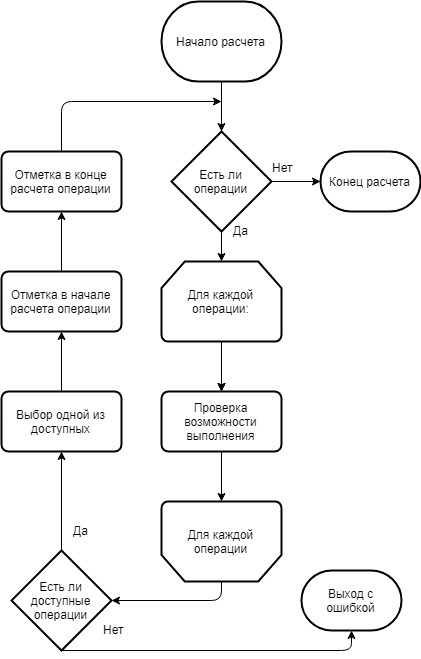
\includegraphics[scale=0.6]{pics/assemblyResSchema.png}
	\caption{Схема работы подсистемы моделирования с ресурсами в процессе расчета оперативного плана}
	\label{fig:assemblyResSchema}
\end{figure}

\indent Проверка производится во время работы системы и именно в этот момент происходит отбор операций в соответствии с внутренним состоянием модели (листинг \ref{lst:lineConstr}).\\
\indent Метод, реализующий логику работы вызывается при выборке операции подсистемой и для каждой вызывается два раза: чтобы отметить состояние модели в начале и в конце расчета операции (см. рисунок \ref{fig:assemblyResSchema}, листинг \ref{lst:lineDone}).

\indent СПП имеет несколько видов ресурсов, одним из которых является модель ресурса сборочной линии.
Она описывает несколько однотипных, то есть с одинаковым числом рабочих постов, физических сборочных линий.
Сборочная линия -- это способ перемещения заготовки от одного рабочего поста к другому; на каждом посту выполняются закрепленные за ним операции.
Под постами понимаются заготовко-места, оснащенные соответствующим технологическим оборудованием и предназначенными для технического воздействия на заготовку для осуществления фиксированного перечня операций.
Объединение нескольких сборочных линий в одну обуславливается упрощением как взаимодействия с подсистемой имитационного моделирования, так и управления моделью, потому как в любом случае (даже когда все линии будут различны по количеству постов) количество линий в модели будет всегда меньше либо равно количеству физических сборочных линии.
Благодаря такому объединению представляется возможным инкапсулировать реализацию распределения заготовок и связанных с ними операций по сборочным линиям внутри модели, а также описывать ситуации, когда один и тот же рабочий может перемещаться между линиями в пределах одного поста.

\begin{figure}[ht]
	\centering
	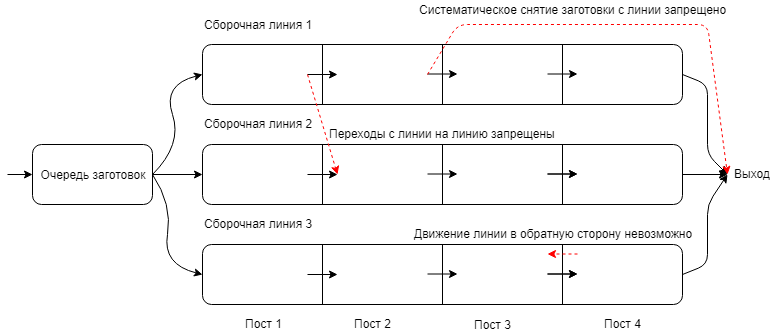
\includegraphics[width=\linewidth]{pics/assemblyMain.png}
	\caption{Схема модели ресурса с вариантами перемещения заготовки внутри}
	\label{fig:assemblyMain}
\end{figure}

\indent Главным назначением модели, как и реальной сборочной линии, является ограничение перемещения продукции внутри ресурса (см. рисунок \ref{fig:assemblyMain}), и моделирование работы физического сборочного конвейера.
С одной стороны ограничивается перемещение между сборочными линиями: к какой продукт был привязан, на той он и останется до окончания выполнения всех операций, относящихся к данному продукту и привязанных к постам данной сборочной линии.
С другой -- перемещение продукции между рабочими постами: продукт должен двигаться последовательно с поста на пост (см. рисунок \ref{fig:assemblyMain}).\\

\begin{lstlisting}[caption={Структуры сборочной линии},label={lst:resource},language=Golang]
	// Describes one product.
	type Product struct {
		TypeName     imcore.ProductTypeName
		SerialNumber imcore.ProductSN
	}

	// Describes one station
	type workstation struct {
		isWorking bool		// Is station working?
		isEmpty   bool		// Is station empty? (if station not working this
							// doesn't mean that station is empty).
		time      int64		// Current timestamp of this station.
		product   Product 	// Product on this station.
	}

	// Describes one line.
	type productionLine struct {
		stations []workstation
		maxTime  int64
		minTime  int64
	}

	// AssemblyLine - assembly line resource.
	//	Contains *NumberOfLines* lines that
	//	which consist of same *NumberOfStations*.
	type AssemblyLine struct {
		// NumberOfStations - number of stations for each line.
		NumberOfStations int
		// NumberOfLines - number of lines of this resource.
		NumberOfLines int
		// Operations queue.
		remainEvents []map[Product][]*imcore.ConcreteEvent
		lines        []productionLine // resource lines.
		queue        []Product        // Production queue.
		remain       map[*imcore.ConcreteEvent][]*imcore.ConcreteEvent
		complete     map[*imcore.ConcreteEvent][]*imcore.ConcreteEvent
	}
\end{lstlisting}

\indent Одной из ключевых особенностей практически любой сборочной линии является синхронизация передвижения продукции между постами.
Это означает что, перемещение продукции на сборочной линии будет осуществляться с периодом, равным максимальной длительности выполнения всех операций на постах -- эта длительность называется тактом сборочной линии.
Каждая заготовка сможет сменить пост только после того, как все остальные заготовки будут готовы к смене своих постов.\\
\indent Для реализации необходимого функционала, были введены структуры, описывающие линии, посты, очередь продукции, и очередь операций на каждый пост всех линий.
Каждая линия, моделируемая компонентом, характеризуется временем начала производственного цикла, структурой данный, описывающей набор рабочих постов (в свою очередь описываемые состоянием: "выполняются работы", "простаивает", "отсутствует продукция на посту", технической картой и серийным номером заготовки).

\begin{figure}[ht]
	\centering
	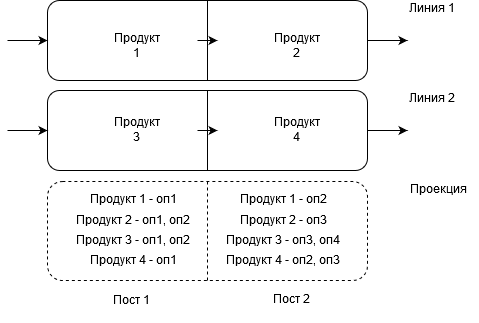
\includegraphics[width=\linewidth]{pics/assemblyBind.png}
	\caption{Схема сборочной линии с очередью операций на посты}
	\label{fig:bind}
\end{figure}

\indent Очередь операций на каждый пост -- структура данных необходимая для динамической привязки операций к линиям модели.
Так как во время привязки операции система не может оценить длительность изготовления продукции, а распределение заготовок происходит до начала работы, может сложиться ситуация, когда одна из линий будет работать намного дольше или меньше по сравнению с другими линиями, что приведет к простою производства.
Следовательно необходимо, не привязывая операцию к определенной линии, обозначить к какому посту она относится (см. рисунок \ref{fig:bind}).
Это является основной задачей разработанной структуры -- она содержит то же количество постов, что и остальные линии, но не описывает какую либо физическую сборочную линию, а является очередью операций всех постом для всех линий.
Внутри каждого поста данной очереди находится хэш-таблица\footnote{структура данных, позволяющая хранить пары (ключ, значение) и выполнять три операции: операцию добавления новой пары, операцию поиска и операцию удаления пары по ключу}, в которой ключом является конкретная единица продукции (характеризующаяся типом продукции и серийным номером), а значением -- список операций, который необходимо выполнить над данной заготовкой на посту.

\begin{figure}[ht]
	\centering
	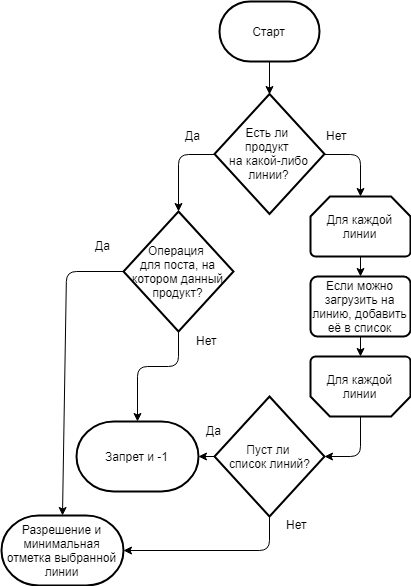
\includegraphics[width=0.7\linewidth]{pics/assemblyConstrain.png}
	\caption{Схема проверки возможности выполнения операции}
	\label{fig:constrain}
\end{figure}

\indent Во время выполнения система, для определения возможности выполнения операции опрашивает все линии с целью определения возможности выполнения данной операции и местонахождения продукта (рисунок \ref{fig:constrain}, листинг \ref{lst:lineConstr}):

\begin{itemize}
	\item при отсутствии продукта на всех линиях:
		\begin{enumerate}
			\item[1)] инициируется проверка всех линий на возможность загрузки первого поста (то есть пуст ли он, листинг \ref{lst:lineCan});
			\item[2)] из получившегося списка линий (если количество больше нуля, иначе переход к \ref{itm:point4} пункту) выбирается линия, временная отметка которой является наименьшей среди всех доступных линий;
			\item[3)] возвращается разрешение на выполнение данной операции и временная метка, выбранная на предыдущем шаге;
			\item[\mylabel{itm:point4}{4})] иначе (количество линий равно нулю) возвращается запрет на выполнение данной операции на текущей итерации.
		\end{enumerate}
	\item если продукт находится на какой-либо линии (листинг \ref{lst:lineFind}), то производится опрос очереди операций:
		\begin{enumerate}
			\item[1)] при нахождении нужной операции на посту, на котором находится в данный момент продукт, возвращается разрешение на выполнение и временная метка, с которой может производиться данная операция;
			\item[2)] иначе возвращается запрет выполнения.
		\end{enumerate}
\end{itemize}

\indent Подсистема имитационного моделирования последовательно переберет все доступные на данной итерации операции и выберет одну из тех, что получили разрешение от всех моделей ресурсов на выполнение.
Если таковых не будет, то система известит о невозможности дальнейшей работы вследствие логической ошибки во входных данных.
В ином случае произойдет вызов метода для того, чтобы отметить состояние модели в начале выполнения операции.
При этом, если продукт не был загружен на линию, то он будет загружен, иначе произойдет проверка на возможность сдвига линии.\\
\indent Во второй раз метод будет вызван для того, чтобы отметить окончание операции -- это означает что данная операция будет удалена из проекции, временная метка поста будет изменена с учетом длительности операции, и, если операций на данном посту для данного продукта не осталось, то состояние поста изменится на ``готов к сдвигу линии'' и будет совершена проверка возможности сдвига линии.

\begin{figure}[ht]
	\centering
	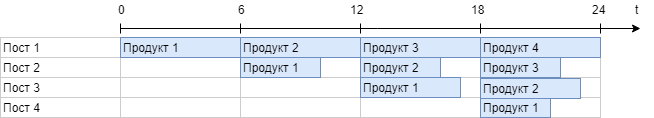
\includegraphics[width=\linewidth]{pics/assemblyDiagram.png}
	\caption{Диаграмма, изображающая сдвиг линии}
	\label{fig:lineDiagram}
\end{figure}

\indent Сдвиг линии -- процесс, при котором все посты на сборочной линии передают свою заготовку на следующий пост и принимают заготовку с предыдущего.
Данный процесс происходит одновременно для всех постов, не может быть разделен или проигнорирован каким-либо постом и выполняется после получения от всех постов сигнала о готовности к сдвигу.
При этом происходит синхронизация постов, то есть все посты, и, соответственно вся линия, получают одну временную отметку -- сумма предыдущей отметки начала рабочего такта и длительности текущего рабочего такта линии.
С этой отметки начинается отсчет следующего такта (см. \ref{fig:lineDiagram}, листинг \ref{lst:lineMove}).

% \begin{figure}[ht]
% 	\centering
% 	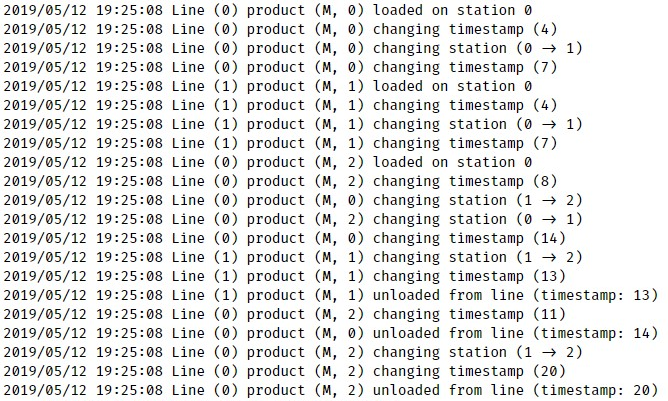
\includegraphics[width=\linewidth]{pics/assemblyResult.png}
% 	\caption{Журнал с результатами работы модели ресурса сборочной линии}
% 	\label{fig:lineResult}
% \end{figure}

\begin{lstlisting}[caption={Интерфейс ресурса},label={lst:assemblyLog},language=Golang]
	2019/05/31 23:10:35 Line (1) product (M, 1) loaded on station 0
	2019/05/31 23:10:35 Line (1) product (M, 1) changing timestamp (4)
	2019/05/31 23:10:35 Line (1) product (M, 1) changing station (0 -> 1)
	2019/05/31 23:10:35 Line (1) product (M, 1) changing timestamp (7)
	2019/05/31 23:10:35 Line (2) product (M, 2) loaded on station 0
	2019/05/31 23:10:35 Line (2) product (M, 2) changing timestamp (4)
	2019/05/31 23:10:35 Line (2) product (M, 2) changing station (0 -> 1)
	2019/05/31 23:10:35 Line (2) product (M, 2) changing timestamp (7)
	2019/05/31 23:10:35 Line (1) product (M, 3) loaded on station 0
	2019/05/31 23:10:35 Line (1) product (M, 3) changing timestamp (8)
	2019/05/31 23:10:35 Line (1) product (M, 1) changing station (1 -> 2)
	2019/05/31 23:10:35 Line (1) product (M, 3) changing station (0 -> 1)
	2019/05/31 23:10:35 Line (1) product (M, 1) changing timestamp (14)
	2019/05/31 23:10:35 Line (2) product (M, 2) changing station (1 -> 2)
	2019/05/31 23:10:35 Line (2) product (M, 2) changing timestamp (13)
	2019/05/31 23:10:35 Line (2) product (M, 2) unloaded from line (timestamp: 13)
	2019/05/31 23:10:35 Line (1) product (M, 3) changing timestamp (11)
	2019/05/31 23:10:35 Line (1) product (M, 1) unloaded from line (timestamp: 14)
	2019/05/31 23:10:35 Line (1) product (M, 3) changing station (1 -> 2)
	2019/05/31 23:10:35 Line (1) product (M, 3) changing timestamp (20)
	2019/05/31 23:10:35 Line (1) product (M, 3) unloaded from line (timestamp: 20)
\end{lstlisting}

\indent Для наглядного представления процессов происходящих в данной модели, на каждой итерации работы создается несколько записей в журнал для отслеживания состояния модели в данный момент -- по ним можно отследить некорректное поведение, либо просто узнать причины, по которым подсистема имитационного моделирования отработала именно в данной последовательности (естественно при условии работы с моделью ресурса сборочной линии).
На листинге \ref{lst:assemblyLog} видно, что модель ресурса охватывает две линии (1 и 2) физических конвейеров и работает с тремя продуктами типа ``М'' (1, 2 и 3).
Также в данном журнале видны все передвижения продуктов между постами (station), все изменения временных меток и результирующие метки отгрузки с последних постов.\\
\indent По завершении основной разработки, было произведено как ручное тестирование (просмотром логов в поисках ошибок работы, листинг \ref{lst:assemblyLog}), так и автоматизированное с написанием модульных (для проверки самой модели) и интеграционных тестов (для проверки работы с подсистемой имитационного моделирования и другими моделями ресурсов) -- которые показали правильную работу во всех рассмотренных случаях.

\indent В результате проведенного тестирования (25 тестов), покрытие кода составило 84.3\%, что отражено в листинге \ref{lst:passLine}.

\begin{lstlisting}[caption={Тестовое покрытие кода},label={lst:passLine}]
	PASS
	coverage: 84.3% of statements
	ok	nitta.io/yamp/imcore/resource	1.041s	coverage: 84.3% of statements
	Success: Tests passed.
\end{lstlisting}
